\begin{figure}[t]
    \centering
    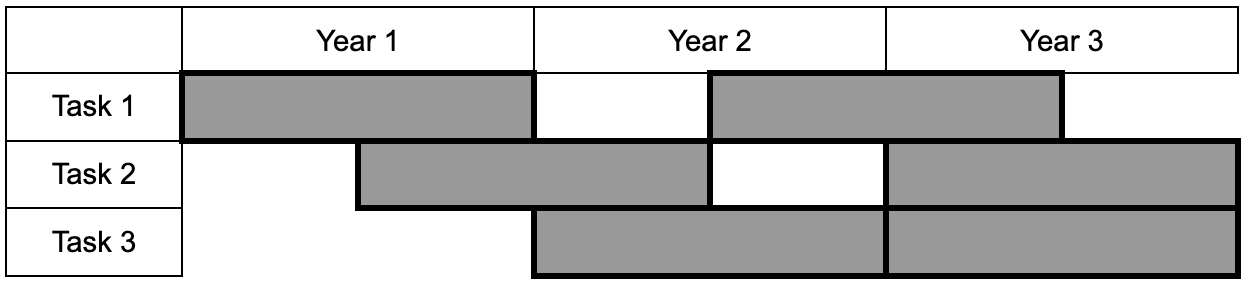
\includegraphics[width=0.6\linewidth]{figures/timeline.png}
    \caption{Timeline.}
    \label{fig:timeline}
\end{figure}


\section{Management Plan and Timeline}\label{sec:management}

PI Huang will manage all aspects of this project. The project will involve
graduate students and research staff who will help with the implementation of
the project, as well as sustaining the software over time and transferring the
data and systems to other organizations, as described in
Section~\ref{sec:impacts}. We envision that the tasks of this project will
proceed roughly in phases, in order, with some overlap as appropriate. As illustrated in Figure~\ref{fig:timeline}, we will proceed with Tasks 1, 2, and 3 in order, with some overlap in the middle to allow for continuous improvement and feedback. Once we deploy, we will return to Task 1 and Task 2 again to further improve the system based on preliminary deployment in Task 3. We hope to achieve full-scale deployment by the end of the third year, while continuously running user studies (Task 1) and fine-tuning our traffic annotations and anomaly detection (Task 2).
